\chapter{Proposta} \label{cap:cap4}

A proposta de uso do dispositivo háptico para treinamento de anestesia raquidiana apresentada nesta tese envolve a criação de um simulador que permite o treinamento de aprendizes na técnica de anestesia raquidiana utilizando um ambiente virtual de treinamento.
Este ambiente virtual foi desenvolvido utilizando o motor de jogo Unity3D \cite{UnityTechnologies2020} com uso de \textit{plugin} para o dispositivo háptico \textit{Geomagic Touch}®, os \textit{scripts} foram desenvolvidos em C\#. O código foi desenvolvido como uma evolução do simulador epidural desenvolvido por \textcite{Brazil2017} levando em consideração que diversas funcionalidades existentes foram estendidas e modificadas. O foco passou de anestesia epidural para anestesia raquidiana. Um novo modelo 3D foi construído para representar fielmente as camadas do corpo humano, para isto as formas e volumes das camadas foram baseadas num corpo 3D interativo cientificamente preciso \cite{BioDigitalInc2019}. Adicionalmente a isto as principais camadas (tecidos do corpo) foram programadas com um margem de crescimento individual onde o crescimento da camada mais interna "empurra" as camadas mais externas pra fora. Isto foi feito para possibilitar uma maior variabilidade de cenários e para que estes sejam visualmente coerentes quando a transparência das camadas for aplicada. Além da possibilidade de se crescer individualmente cada camada, também é possível que todas as camadas cresçam de forma homogênea através da aplicação de matrizes de transformação. 

\section {Desenvolvimento do ambiente de treinamento} 

O modelo 3D para o tronco do corpo feminino (área onde é feita a punção) foi desenvolvido usando o software de modelagem e criação \textit{3ds Max} \cite{Autodesk}. Exemplos das suas diversas camadas internas podem ser observados na figura \ref{fig:modelo3Dcorpo}. 

\begin{figure}[ht!]
    \centering
        \begin{tabular}{cc}
        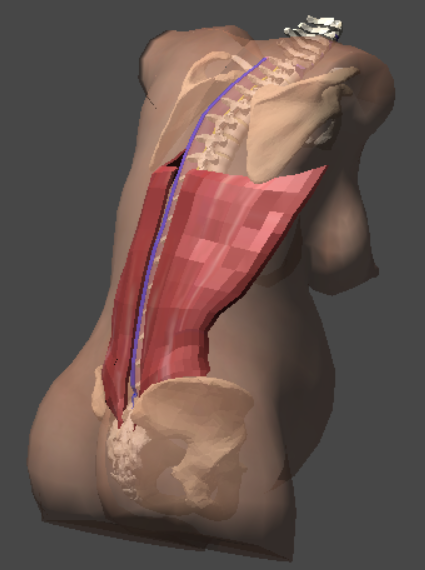
\includegraphics[width=0.4\linewidth]{capitulos/figuras/modelo corpo 3d.PNG} & 
        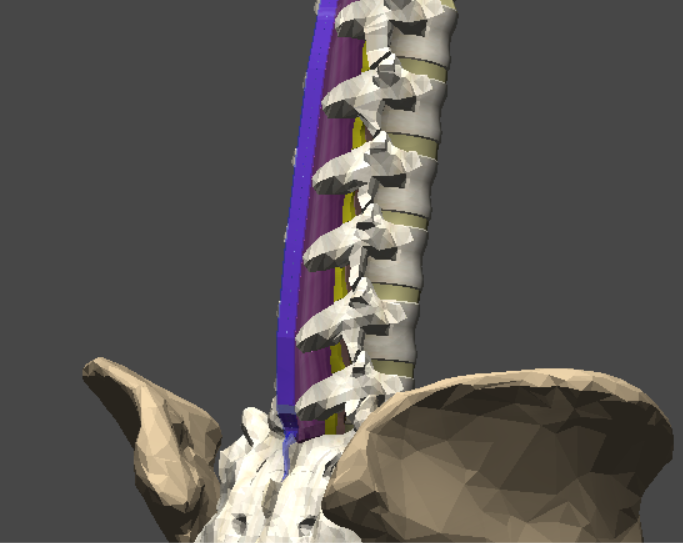
\includegraphics[width=0.6\linewidth]{capitulos/figuras/modelo corpo 3d - coluna vertebral, ligamentos supra, interespinhoso and flavum.PNG} 
        \\
        (a) & (b)
        \end{tabular}
    \caption{Modelo 3D de corpo de mulher grávida desenvolvido com diferentes níveis de transparência \cite{Melo2021}: (a) Corpo, ossos e músculos (b) Osso, vértebras e ligamentos.}
    \label{fig:modelo3Dcorpo}
\end{figure}

Como comentado anteriormente foram criados controles para crescimento das principais camadas do corpo. Primeiro é necessário iniciar um projeto na \textit{Unity} e importar o modelo 3D. Com isto estes controles ficam acessíveis via código nas diversas linguagens suportadas pela \textit{Unity} assim como via interface da \textit{Unity}. Para a nossa solução onde precisávamos fazer modificações em tempo de execução optamos pelo acesso através do código em C# para fazer as modificações de tamanho das camadas (quando necessário). 

Para que seja possível fazer a interação com o dispositivo háptico \textit{Geomagic Touch®} o driver \textit{Open Haptics Touch Device} precisa ser instalado na máquina onde o dispositivo será usado, este driver pode ser encontrado no endereço eletrônico da empresa responsável pela produção e comercialização deste dispositivo háptico \cite{3DSystemsTouch2018}. Para que este dispositivo possa ser utilizado na \textit{Unity} optamos pela instalação do \textit{Haptic Plug-In For Unity3D} \cite{Poyade2014}. Este \textit{plugin} contém exemplos que exploram as funcionalidades e dos dispositivos hápticos suportados. As características específicas que foram utilizadas nos experimentos são comentadas no capítulo~\ref{cap:cap5}. No ambiente de treinamento utilizamos configurações similares as dos experimentos ajustadas de acordo com cada corpo de paciente sendo simulado. 

Foi incluída uma visão lateral da cena (Figura~\ref{fig:posicaoSentadaComTransparencia}) a partir do \textit{feedback} de um anestesista sobre pontos de melhoria da ferramenta de treinamento para possibilitar um outro ponto de vista do procedimento sendo efetuado. Esta característica ajuda não só o indivíduo em treinamento mas também pessoas que possam assistir o treinamento ao vivo ou ainda gravações deste que pode ser disponibilizado futuramente. Nesta mesma imagem fizemos também a demonstração da visibilidade das camadas interiores do corpo (que é exibida ao pressionar usando o mouse o botão "visibilidade" no menu do lado esquerdo). Esta funcionalidade pode ser utilizada por iniciantes nos seus primeiros treinamentos.  

\begin{figure}[ht!]
    \centering
    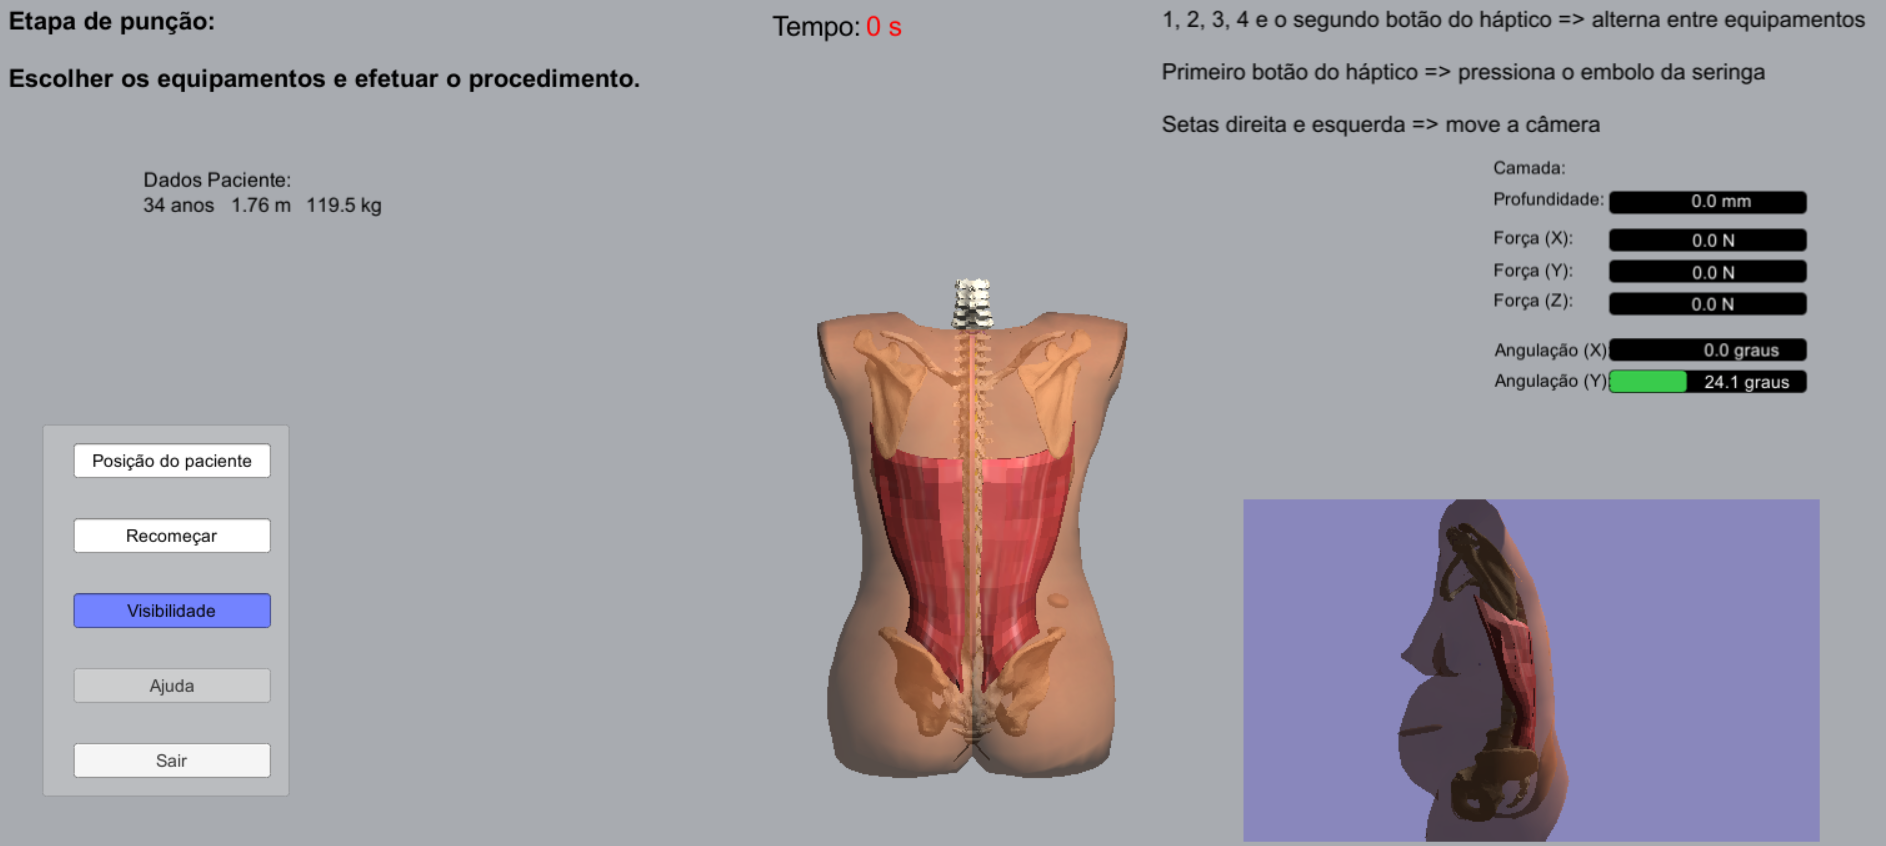
\includegraphics[width=0.9\linewidth]{capitulos/figuras/sistema posicao sentada com transparencia.png} 
    \caption{Visão geral do sistema com tronco de paciente centralizada na tela na posição sentada. Do lado inferior direito a visão lateral desta mesma parte do corpo.}
    \label{fig:posicaoSentadaComTransparencia}
\end{figure}

Uma outra opção de execução do procedimento incluída foi a possibilidade de mudança de posição da paciente (Figura~\ref{fig:posicaoDeitada}) que além da posição sentada (original e mais comum) agora também permite que o procedimento seja feito com ela deitada (estas são as duas posições em que ocorre o procedimento de raquianestesia \ref{sec:anestesiaRaquidiana}).

\begin{figure}[ht!]
    \centering
    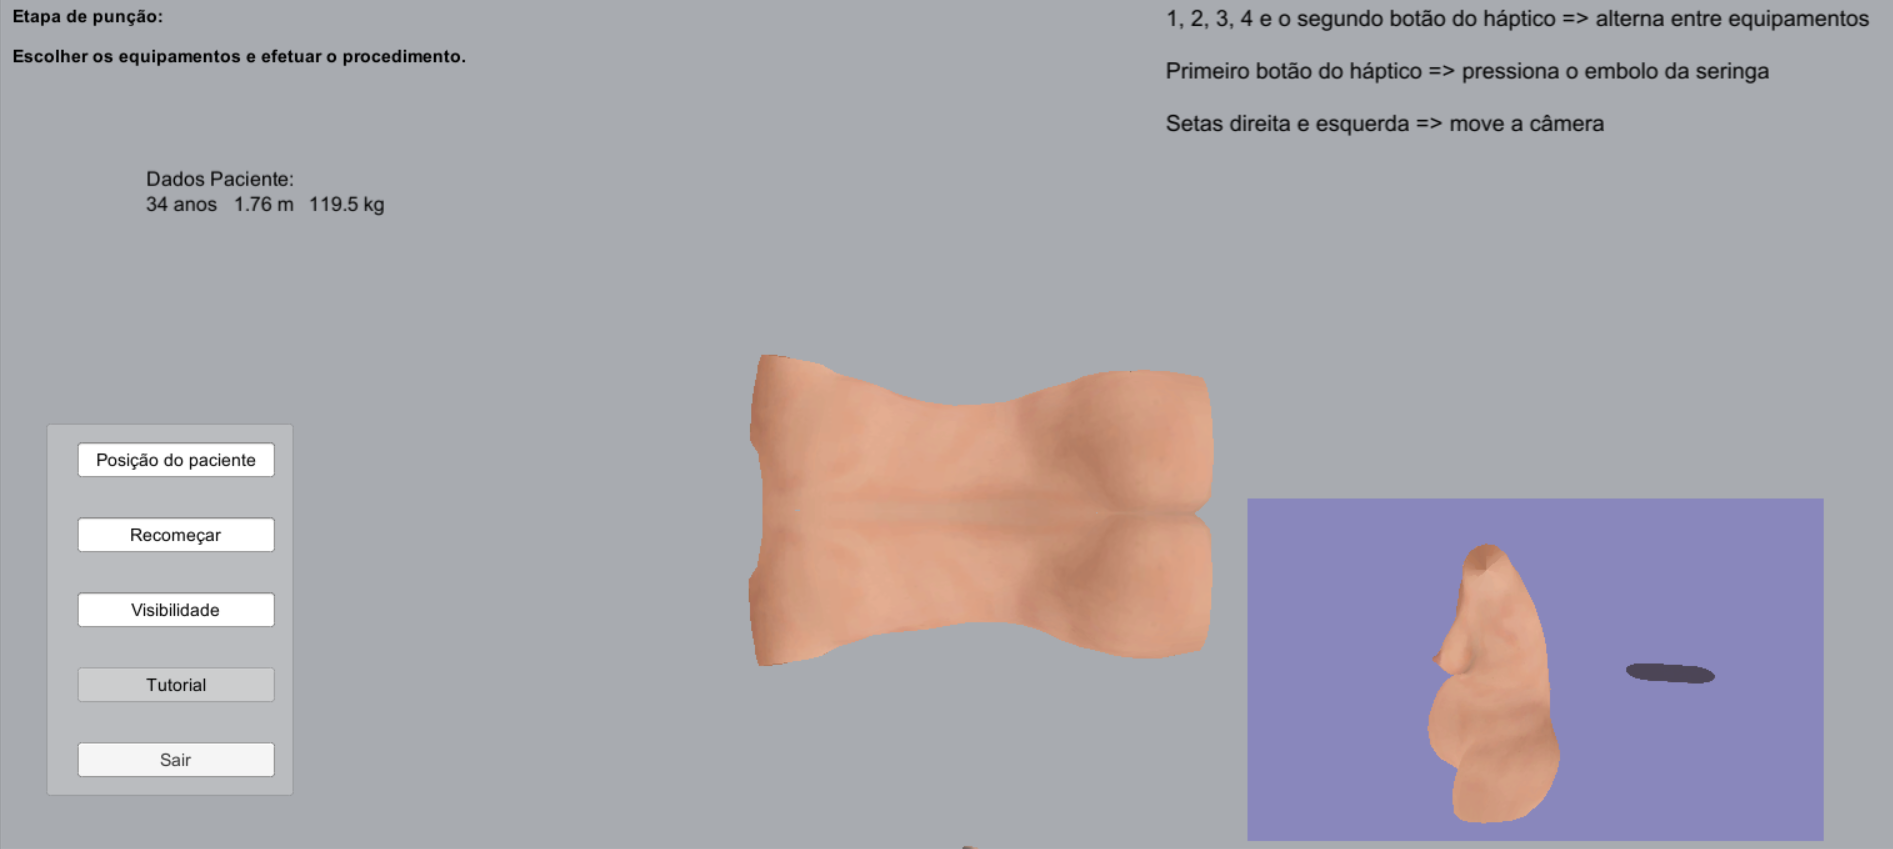
\includegraphics[width=0.9\linewidth]{capitulos/figuras/sistema posicao deitada.png} 
    \caption{Visão geral do sistema com tronco de paciente na posição deitada.}
    \label{fig:posicaoDeitada}
\end{figure}

\subsection {Simulação de pacientes virtuais}

======
 MOSTRAR VARIAÇÕES DO CORPO PELAS TRANSFORMAÇÕES EXISTENTES
======